\begin{example}[\quad \large Közvetelen érzékelők 1.]

Egy kapcsolóüzemű tápegység szűretlen kimenő feszültségét nagy pontossággal és jó dinamikával szeretnénk mérni. A kimenet és a vezérlő elektronika tápja egy ponton összeköthető. Javasoljon érzékelési módszert és méretezze az érzékelőt! ($Ui=0..100V, Uo=0..5V$, előírt pontosság 1\%, az A/D váltó bemeneti árama 1uA(max), bemeneti kapacitása 50pF(max.).

\tcbline
\vspace{1mm}

\solution
\end{example}
Első lépésben gyűjtsük ki a szükséges paramétereket, a jelölések értelmezéséhez a \ref{fig:volt_div_sol}. ábra szolgál segítségül:
\begin{equation}
\begin{aligned}{}
    U_{in} &= 0..100\; V; \\
    U_o &= 0..5\; V; \\
    C_{AD} &= 50\; pF; \\
    I_{AD} &= 1\; \mu{}A; \\
    \alpha{} &= 1\; \%; \\
\end{aligned}
\end{equation}

Ezek után meghatározzuk a feszültésgosztáshoz székséges ellenállások mértékét a feszültésgosztó képlettel.

\begin{equation}
\begin{aligned}{}
    U_{o} &= U_{in} \cdot \frac{R_2}{R_1 + R_2} \\
\end{aligned}
\end{equation}

Mivel ebben az egyenletben két ismeretlen van, így a megoldáshoz $R_1$ és $R_2$ értéke közül az egyiket nekünk kell megválasztanunk. A gyakorlatban ezeket az ártákeket általában úgy választjuk meg, hogy a feszültésgosztó árama kelleően kicsi legyen, elkerülve a nagy teljesítmény disszipációt, viszont ne túl kicsi ahhoz, hogy túlságosan zavarérzékeny legyen. Ebben a feladatban meg van adva az elvárt pontásság $\alpha{} = 1 \%$, illetve az AD váltó által felvett áram maximális értéke $I_{AD} = 1 \mu{}A$. Ezt értelmezhetjük úgy, hogy az AD váltó áramfelvétele, maxmim $1\%$ mértékben változtathatja meg a feszültségosztó áramát, tehát $R_2$ áramának legalább a 100 szorosának kell lennie $I_{AD}$-nak.

\begin{equation}
\begin{aligned}{}
    I_{R2} &\geq I_{AD} \cdot \alpha{} \\
    \frac{U_o}{I_{R2}} &\geq \frac{U_o}{I_{AD}} \cdot \alpha{} \\
    R_{2} &\geq \frac{U_o}{I_{AD}} \cdot \alpha{} = \frac{5\;V}{1\;\mu{}A} \cdot \frac{1}{100} = 50\; k\Omega{} \\
    R_2 &= \underline{\underline{50\; k\Omega{}}}
\end{aligned}
\end{equation}

$R_2$ ismeretében már a feladat egyértelmúen megoldható:

\begin{equation}
\begin{aligned}{}
    U_{o} &= U_{in} \cdot \frac{R_2}{R_1 + R_2} \\
    R_{1} &= \frac{U_i \cdot R_2 - U_1 \cdot R_2}{U_o} = \frac{100\;V \cdot 50\; k\Omega{} - 5\; V \cdot 50\; k\Omega{}}{5 \;V} = \underline{\underline{950 \; k\Omega{}}} \\
\end{aligned}
\end{equation}

Innen már nincs más hátra, mint elvégezni a frekvenciakompenzációt.

\begin{equation}
\begin{aligned}{}
    R_1 \cdot C_1 &=  R_2 \cdot C_2 \\
    C_2 &= C_{AD} \\
    C_1 &= \frac{R_2 \cdot C_2}{R_1} = \frac{50\; k\Omega \cdot 50\; pF}{950;\ k\Omega} = \underline{\underline{2,63\; pF}}
\end{aligned}
\end{equation}

Ezzel pedig a feladat el is készült.

\begin{figure}[htb]
\begingroup
\tikzset{}
 \centerline{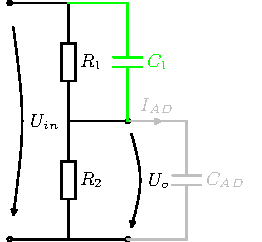
\includegraphics[width=0.4\columnwidth]{.//Figures/Tikz/tikz_voltage_divider.pdf}}
 \endgroup
 \caption{Feszültségosztó}
 \label{fig:volt_div_sol}
\end{figure}